In diesem Kapitel wird die Einbettung des erstellten Prototyps zur Erkennung und Ausmessung von Makulaödemen in die Software des Uniklinikums beschrieben.
\section{Architektur}

Die Fidus Software schreibt Ordner mit Patientenbildern auf einen Server.

Das Skript für den Prototypen hat die Aufgabe, zu scannen ob neue Patientenbilder auf dem Server vorhanden sind und wenn ja, diese dem Klassifikationsmodell zu übergeben, deren positiven Output von dem Segmentierungsmodell segmentieren zu lassen um letztlich das Vorhandensein von Ödemen in einem Auge, sowie deren Gesamtgröße, in eine JSON Datei zu schreiben und hinter sich aufzuräumen, indem es die Bilder samt Ordner löscht.

Fidus wiederum verwertet diese JSON Dateien und schreibt die Informationen in die Patientenkartei.

Dieser Workflow ist in Abb. \ref{fig:prototyp} visualisiert. Da wie später in diesem Kapitel beschrieben das Klassifizierungsmodell nicht als Vorfilter verwendet wurde, entfällt der rot dargestellte Teil in der finalen Implementierung.

\begin{figure}[ht!]
\centering
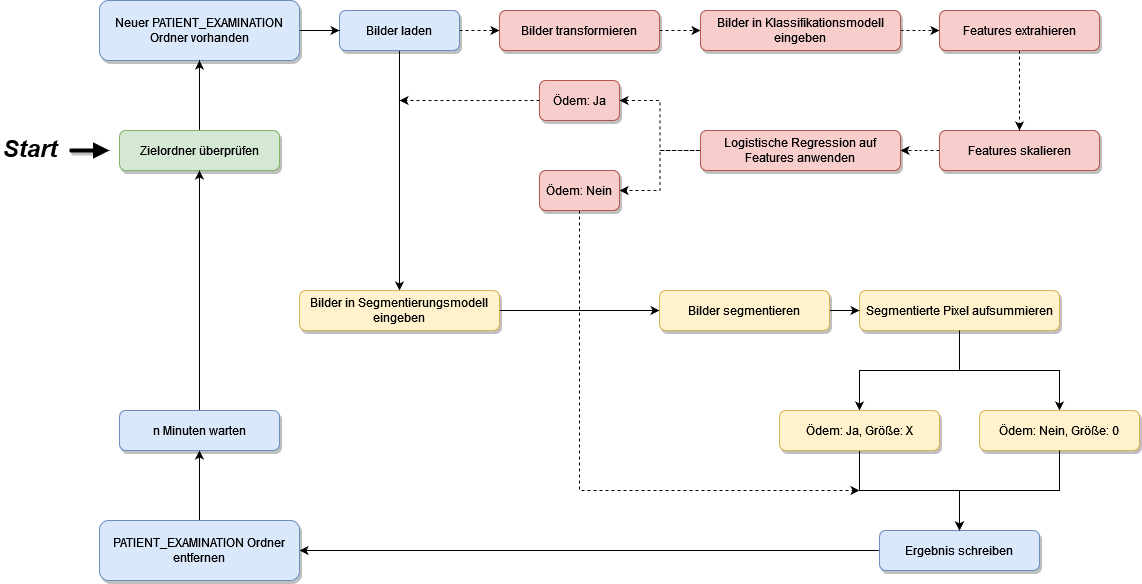
\includegraphics[width=0.75\textwidth]{./pic/Prototyp/flowchart.png} 
\caption{\label{fig:prototyp}Architektur des Skriptes für den Prototypen. - \textit{erstellt mit}: \cite{23}}
\end{figure}

\section{Entscheidung gegen die Klassifikation als Vorfilter}

Die Klassifikation als Vorfilter verbessert in der Theorie die Spezifität, indem sie Möglichkeiten für falsch positive verringert, was in diesem Fall jedoch unerwartet teuer in der Sensitivität schien und weitaus ausführlicher analysiert werden muss, idealerweise mit identischen Trainings- und Testdatensätzen auf beiden Modellen (bei der Segmentierung nur die positiven Bilder dieser Datensätze), um Gewinne in der Spezifität und Verluste in der Sensitivität quantifizieren zu können.

Es fiel auf, dass bei der Evaluation der Klassifikationsmodelle noch mehr Wert auf die Sensitivität gelegt werden sollte, als bereits getan. Das liegt daran, dass selbst wenn beispielsweise zwei Modelle wie in Abbildung \ref{pic:Prefilter_TP} mit einer Sensitivität von 0.9 für sich alleine gestellt recht gut performen, die Kombination dieser wiederum einige echt positive Resultate verliert allein dadurch, dass die 90\% der korrekt positiv klassifizierten des einen Modells nicht zwangsläufig deckungsgleich mit denen des zweiten Modells sind und somit weitere bis zu 10\% Schwund entstehen können. Hierdurch würde man im Gesamtmodell letztlich gerade mal eine Sensitivität zwischen 0.8 und 0.9 erreichen und dementsprechend weniger als nur das Segmentierungsmodell alleine mit seinen 0.9.

\begin{figure}[H]
\centering
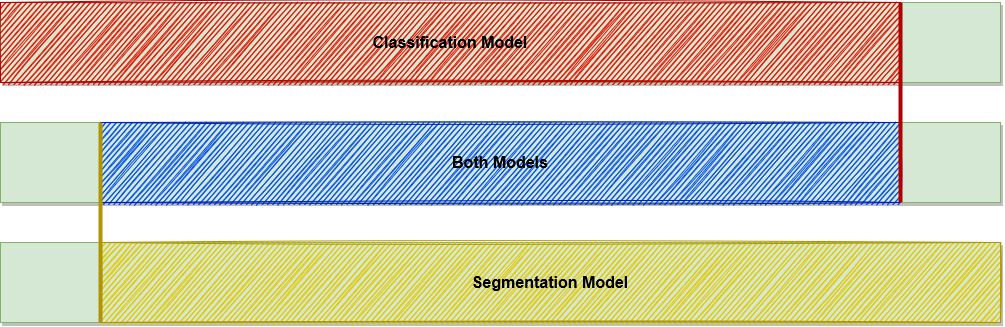
\includegraphics[width=0.5\textwidth]{./pic/Prototyp/prefilter.png}
\caption{\label{pic:Prefilter_TP}Der Worst-Case eines Klassifikationsmodells (rot) mit einer Sensitivität von 0.9, eines Segmentierungsmodells (gelb) mit einer Sensitivität von 0.9, sowie die Kombination dieser (blau) mit einer Sensitivität von 0.8, dargestellt als Anteil der echt positiven Bilder (grün). - \textit{erstellt mit}: \cite{23}}
\end{figure}

\section{Umsetzung}

Es gelang eine zufriedenstellende Umsetzung dieser Architektur.

Auf der CPU des Systems der Uniklinik benötigte der Vorgang für 25 Bilder eines Auges in etwa 2 Minuten. Die Ausführung des Skriptes auf dem System der Uniklinik ist in Abbildung \ref{fig:server} zu sehen, die eingebetteten Resultate in die Fidus Software in Abbildung \ref{fig:fidus_beispielpatient}.

\begin{figure}[ht!]
\centering
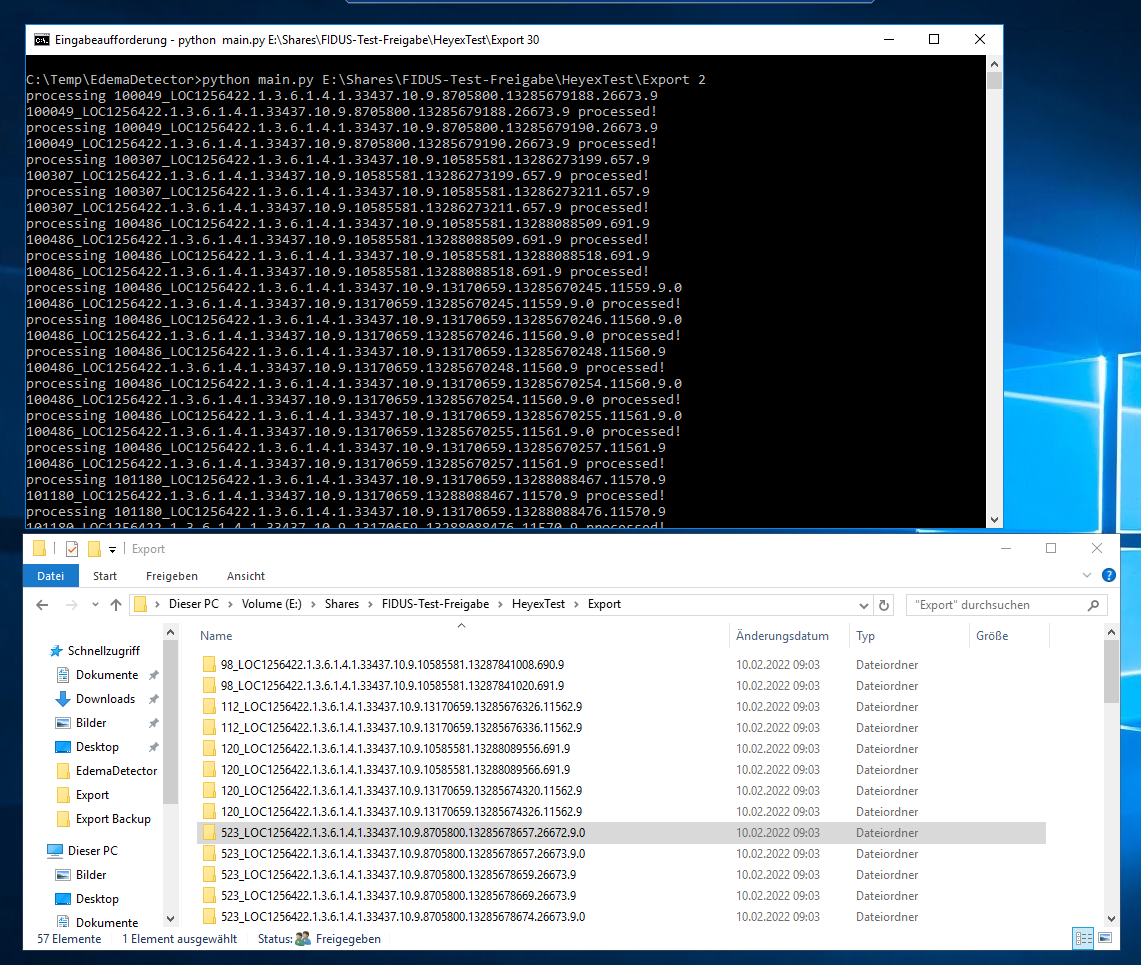
\includegraphics[width=0.75\textwidth]{./pic/Prototyp/server.png} 
\caption{\label{fig:server}Skript für den Prototypen auf dem Server der Uniklinik}
\end{figure}

\begin{figure}[ht!]
\centering
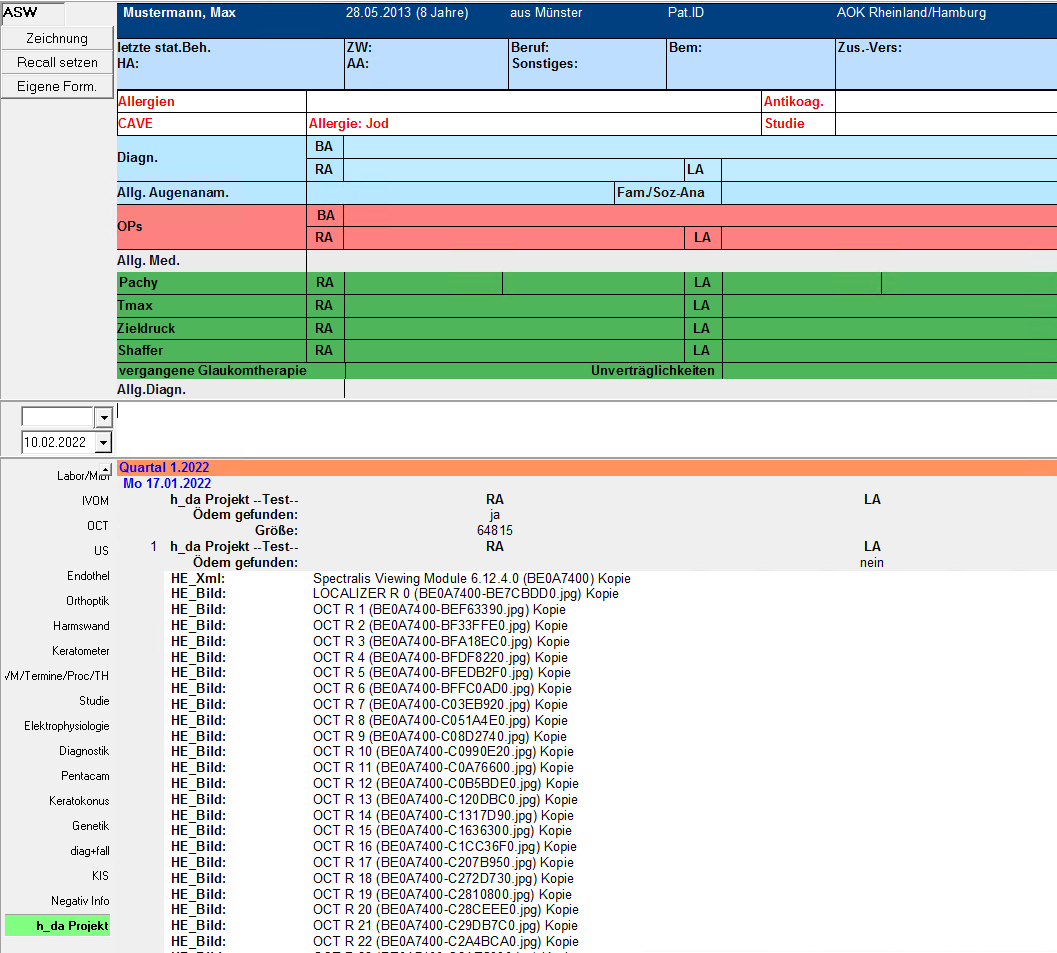
\includegraphics[width=0.75\textwidth]{./pic/Prototyp/fidus.png} 
\caption{\label{fig:fidus_beispielpatient}Beispielpatient in Fidus}
\end{figure}

\section{Performanceverbesserung des Prototypen}

Mit einer besseren Hardware ließe sich die Dauer der Segmentierung deutlich verkürzen. Mit einer CPU des Typs Intel(R) Core(TM) i5-7500 CPU @ 3.40GHz benötigt man zum Beispiel für 25 Bilder eines Auges etwa 36 Sekunden (Faktor 4) oder mit einer GPU des Typs NVIDIA GeForce GTX 1060 6GB etwa 4 Sekunden (Faktor 34). Insbesondere mit einem Klassifikationsmodell als Vorfilter wäre eine Aufrüstung der Hardware empfehlenswert.